\begin{frame}{Video Encoding Frames}
  \begin{figure}
    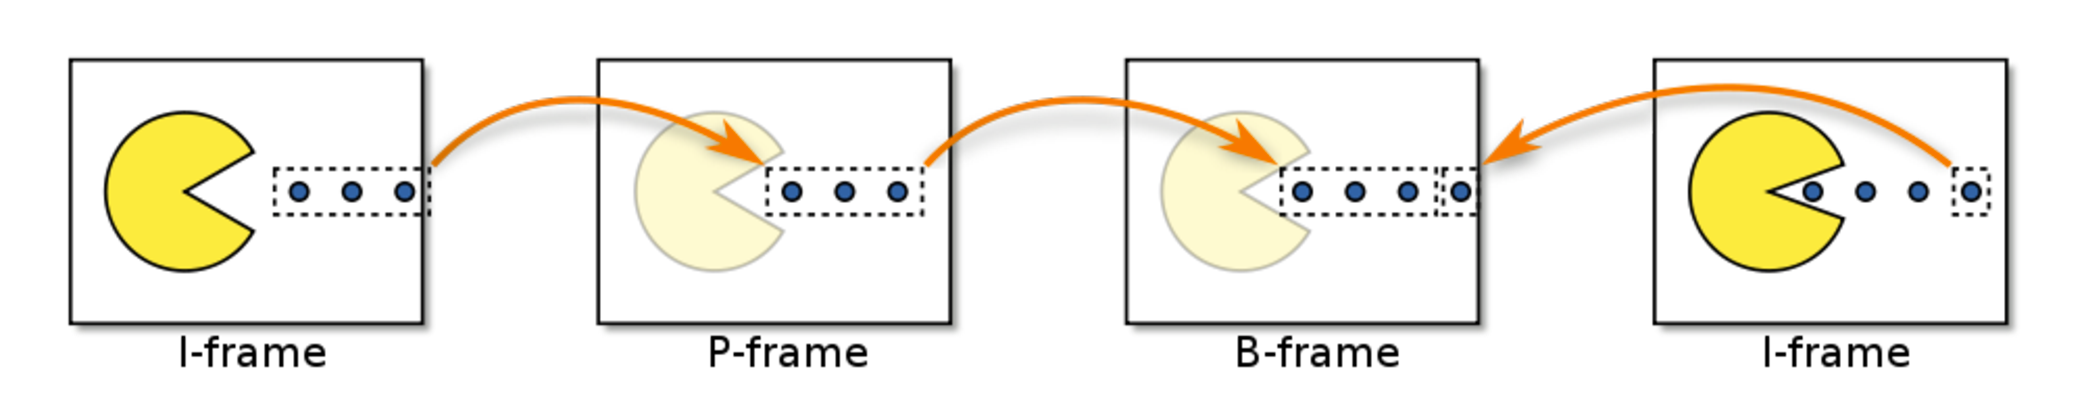
\includegraphics[width=\textwidth]{figures/video-frames.pdf}
    \caption{PC: https://en.wikipedia.org/wiki/Video\_compression\_picture\_types}
  \end{figure}

  \begin{itemize}
  \item \textbf{I-frames} are the least compressible but don't require other
    video frames to decode. I-frames are further compressed with
    quantization.
  \item \textbf{P-frames} can use data from previous frames to decompress
    and are more compressible than I-frames.
  \item \textbf{B-frames} can use both previous and forward frames for data
    reference to get the highest amount of data compression (not an option
    in live streaming).
  \end{itemize}
\end{frame}

\begin{frame}{Bandwidth Fluctuations (Cellular)}
  \begin{figure}
    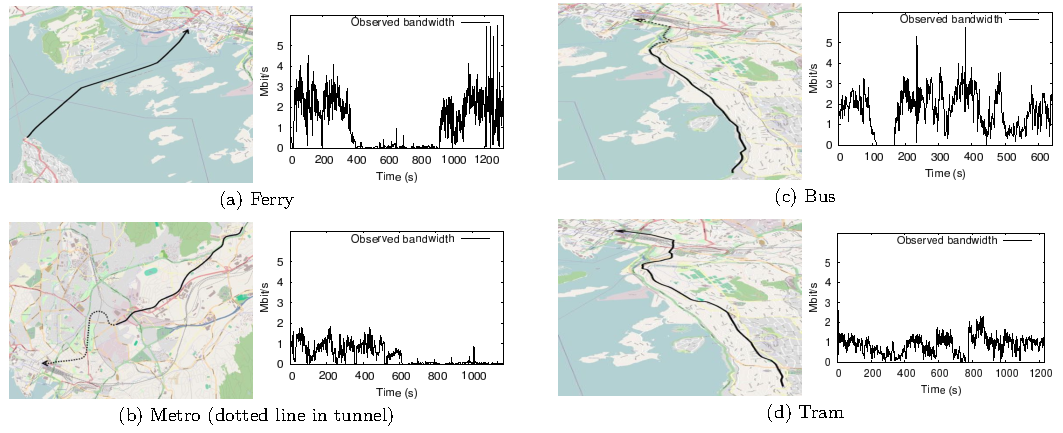
\includegraphics[width=\textwidth]{figures/bandwidth-cellular.pdf}
    \caption{Riiser, Haakon, et al. "A comparison of quality scheduling in
      commercial adaptive HTTP streaming solutions on a 3G network."
      Proceedings of the 4th Workshop on Mobile Video. ACM, 2012.}
  \end{figure}
\end{frame}

\begin{frame}{Bandwidth Fluctuations (WiFi)}
  \begin{figure}
    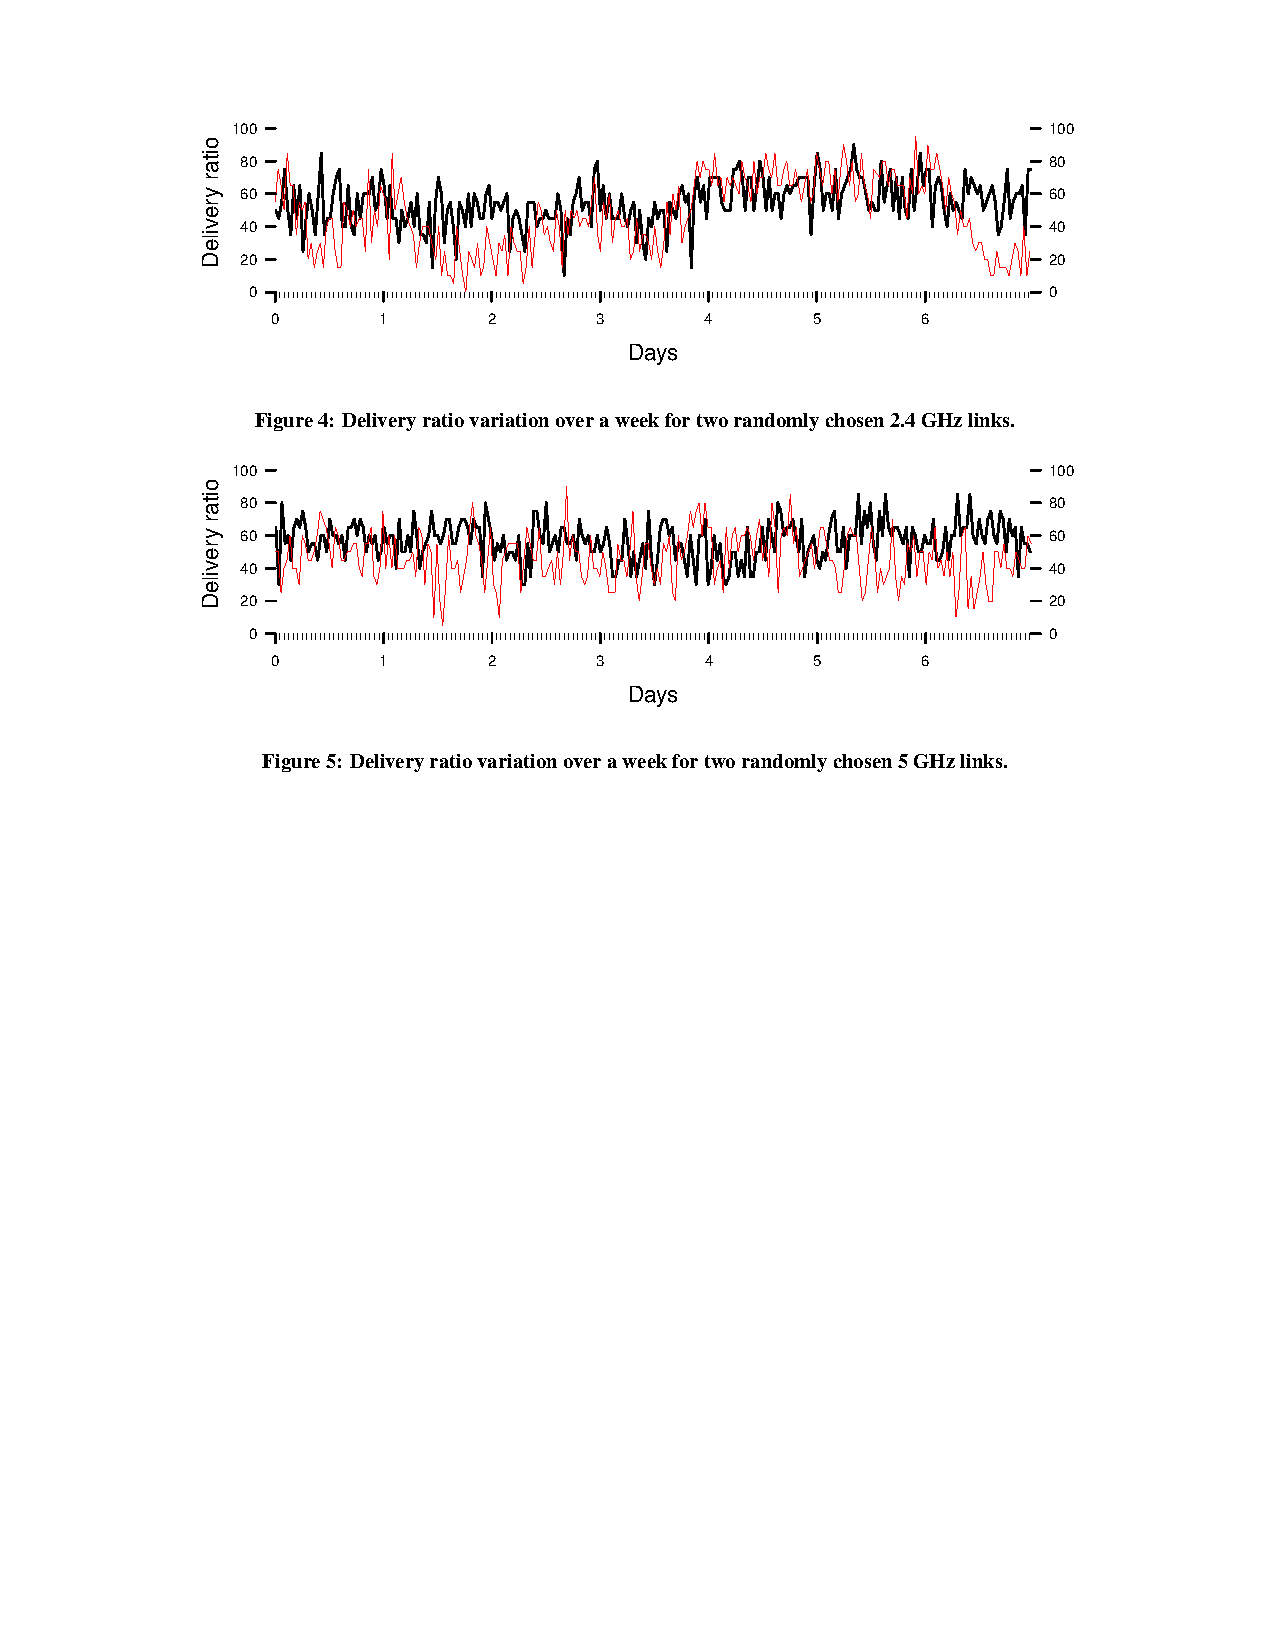
\includegraphics[width=\textwidth]{figures/bandwidth-wifi.pdf}
    \caption{Biswas et al, Cisco Meraki, Large-scale Measurements of Wireless
      Network Behavior, SIGCOMM'15. Two randomly chosen links.}
  \end{figure}
\end{frame}

\begin{frame}{MOT Dataset}
\end{frame}

%%% Local Variables:
%%% mode: latex
%%% TeX-master: "talk"
%%% End:
